\section{Thermodynamic and enhancement-factor consistency}
\label{sec:enhancement-pressure-consistency}

\subsection*{Question}

Does inaccurate liquid \ce{CO2} fugacity explain the retained reactive Case
3C result, or does the absorber combine the reactive liquid state with an
enhancement formulation that uses an inconsistent thermodynamic basis?

\subsection*{Conditions}

The column diagnosis uses parameter document
\texttt{66837...133c63b}.  Pressure comparisons for this exact
document contain 59 source-backed 30 mass-\% MEA states divided into training,
reserved, and temperature-challenge partitions.  The enhancement comparison
holds 21 retained Case 3C liquid states fixed and changes only the named
enhancement and liquid-resistance formulation.  No thermodynamic or kinetic
parameter is fitted to column capture.

A newer speciation-only parameter document from the upstream ePC-SAFT campaign
has SHA-256 \texttt{a2ff7...c26355b}.  Its fitted diameters and
$k_{\ce{CO2},\mathrm{MEA}}$ differ from the column document.  Its pressure
validation is reported separately and is not assigned to the column result.

\subsection*{Results}

\begin{table}[htbp]
    \centering
    \caption{Independent \ce{CO2} partial-pressure comparisons. The geometric mean ratio is $\exp(\overline{\ln(p_{\mathrm{model}}/p_{\mathrm{obs}})})$; the RMS factor reports unsigned scatter.}
    \label{tab:pressure-consistency}
    \begin{threeparttable}
        \small
        \setlength{\tabcolsep}{4pt}
        \begin{tabularx}{0.98\textwidth}{@{}>{\raggedright\arraybackslash}X S[table-format=2.0] S[table-format=2.2] S[table-format=2.3]@{}}
            \toprule
            Parameter document and partition & {Rows} & {RMS factor} & {Mean model/data} \\
            \midrule
            Column document, training & 24 & 2.02 & 1.495 \\
            Column document, reserved & 8 & 2.28 & 1.055 \\
            Column document, temperature challenge & 27 & 2.39 & 0.654 \\
            Newer speciation-only document, independent pressure check\tnote{a} & 55 & {--} & 10.57 \\
            \bottomrule
        \end{tabularx}
        \begin{tablenotes}\footnotesize
            \item[a] Median model/data ratio. All 55 evaluated ratios exceed one; the range is 2.57--16.25.
        \end{tablenotes}
    \end{threeparttable}
\end{table}

The exact column document is not uniformly high.  It overpredicts pressure on
average in the training partition, is nearly unbiased in mean on the small
reserved partition, and underpredicts on average in the temperature challenge.
Its factor-of-two scatter and the absence of an untouched replacement
validation partition prevent a predictive thermodynamic claim.  The newer
speciation-only document performs much worse on pressure, but it was not used
in the column calculation.

\begin{table}[htbp]
    \centering
    \caption{Median fixed-state enhancement and flux ratios relative to the current explicit Luo formulation.}
    \label{tab:enhancement-consistency}
    \small
    \begin{tabularx}{\textwidth}{@{}>{\raggedright\arraybackslash}X S[table-format=1.3] S[table-format=1.3]@{}}
        \toprule
        Formulation & {$E/E_{\mathrm{current}}$} & {$N_{\ce{CO2}}/N_{\mathrm{current}}$} \\
        \midrule
        Current explicit Luo formulation & 1.000 & 1.000 \\
        Explicit Luo without the unexplained divisor & 0.967 & 0.968 \\
        Explicit Putta kinetics without the divisor & 0.954 & 0.955 \\
        Gaspar implicit formulation with legacy Henry resistance & 0.911 & 0.913 \\
        Gaspar implicit formulation with local ePC-SAFT slope & 0.616 & 1.801 \\
        \bottomrule
    \end{tabularx}
\end{table}

\begin{figure}[htbp]
    \centering
    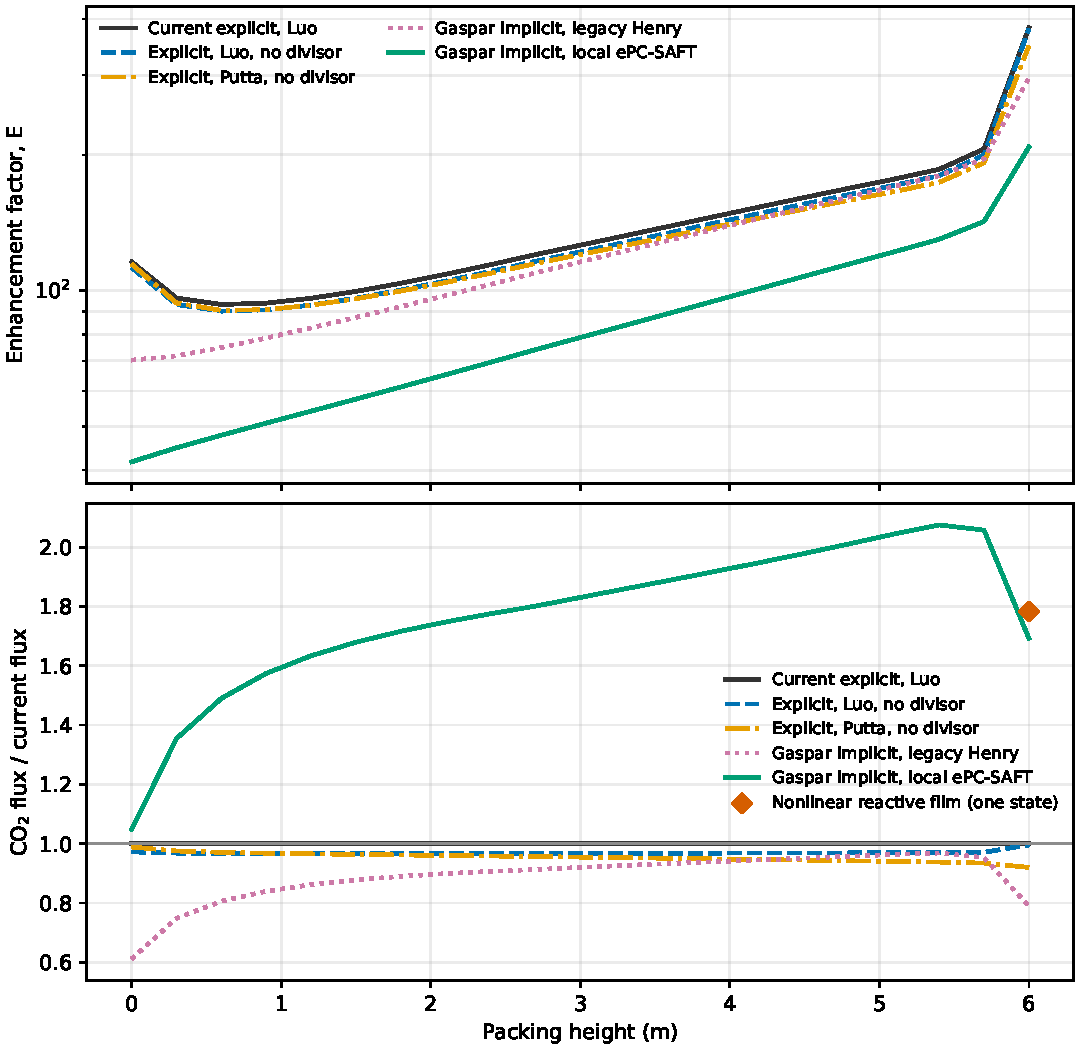
\includegraphics[width=\textwidth]{../../../../analyses/nccc_validation/results/final/figures/retained_reactive_case3c_enhancement_consistency.pdf}
    \caption{Fixed-state enhancement and flux comparisons across 21 retained Case 3C states. Removing the divisor, changing the kinetic source, or solving the implicit equations with the legacy Henry resistance changes median flux by less than 9\%. The ePC-SAFT local slope changes the resistance strongly, but the resulting interface states lie outside the local derivative interval.}
    \label{fig:enhancement-consistency}
\end{figure}

The reactive calculation increases the median molecular-\ce{CO2} mole fraction
by a factor of 4.05.  The current explicit correlation places that molecular
concentration in the denominator of its instantaneous enhancement limit, so
the median enhancement factor falls from 273.9 to 125.1.  This reduction, not
a reduction in the calculated fugacity driving force, dominates the retained
Case 3C transfer decrease.

The local ePC-SAFT fugacity slope is approximately one-third of the legacy
Henry coefficient.  Replacing the legacy resistance with this local slope
therefore lowers $E$ but raises the median fixed-state flux to 1.80 times the
current value.  That apparent increase is not admissible for column use: the
implied interface-to-bulk molecular-\ce{CO2} concentration ratio has median
3.50 and maximum 74.4, far outside the infinitesimal interval used to compute
the slope.

\subsection*{Interpretation}

Two distinct deficiencies remain.  First, the exact column parameter document
has structured partial-pressure error and has not passed independent
thermodynamic validation.  Second, the absorber combines reactive bulk
speciation with an enhancement and resistance formulation derived on the
legacy Henry/speciation basis.  The fixed-state comparisons identify this
basis mismatch as the dominant cause of the calculated Case 3C transfer loss.

The calculations do not demonstrate literal reaction double counting.  Bulk
reaction equilibrium establishes the liquid boundary state, while the
enhancement factor represents reaction and diffusion within the liquid film;
both effects belong in a reactive absorber model.  The present defect is that
the two calculations do not use one consistent fugacity--composition relation
and species basis.  A nonlinear ePC-SAFT film calculation is required to
determine whether the current correlation suppresses or exaggerates transfer.

\subsection*{Limitations}

The enhancement experiment holds the 21 bulk states fixed and does not predict
a new column profile or capture.  The local-slope case is an extrapolation
diagnostic, not a candidate correlation.  The pressure partitions for the
column document were used during earlier model selection and therefore do not
provide untouched validation.  The newer upstream parameter document must not
be substituted without repeating the column calculation and its pressure,
speciation, and transport checks.

\FloatBarrier
